\documentclass{patmorin}
\usepackage{amsopn,amsthm,amsmath,graphicx}
\usepackage{pat}

\DeclareMathOperator{\cn}{cr}

\newcommand{\const}{268.19}

\title{Ghost Chimneys}
\author{Barbados 2010 Gang}

\begin{document}
\maketitle

\begin{abstract}
A set $S$ of points in $\R^2$ is an $(i,t)$ set of ghost chimneys
if there exists lines $H_0,\ldots,H_{t-1}$ such that the orthogonal
projection of $S$ on $H_j$ consists of exactly $i+j$ distinct points.
In this paper we give upper and lower bounds on the maximum value of $t$
in an $(i,t)$ set of ghost chimneys.
\end{abstract}

\section{Introduction}

We consider the following problem:  Given an integer $i$, what
is the maximum value $t(i)$ such that there exists a set of points
$S\subset\R^2$ and a set $H_0,\ldots,H_{t-1}$ of lines where, for each
$j\in\{0,\ldots,t(i)-1\}$, the orthogonal projection of $S$ onto $H_j$
consists of exactly $i+j$ distinct points.  We prove the following result:

\begin{thm}\thmlabel{main}
For any integer $i\ge 1$,  $2i -1 \le t(i) \le 123.33i$.
\end{thm}

\thmref{main} is an immediate consequence of \lemref{lower-bound} and
\lemref{upper-bound}, which are proven in the next two sections. 

\section{The Lower Bound}

\begin{lem}\lemlabel{lower-bound}
For each integer $i\ge 1$, there exists a set $S=S(i)$ of $3i-1$
points and a set $H_0,\ldots,H_{2i-1}$ of lines such that, for each
$j\in\{0,\ldots,2i-1\}$, the orthogonal projection of $S$ onto $H_j$
has exactly $i+j$ distinct values.
\end{lem}

\begin{proof}
The point set $S$ consists of the points of a $i\times 3$ grid with the bottom-right corner removed (see \figref{lower-bound}).  For even $j$, $H_j$ is a line of slope $j/2$.  For odd $j$, $H_j$ is a line of slope $-(j+1)/2$.
\begin{figure}
  \begin{center} 
    \begin{tabular}{cc}
      & 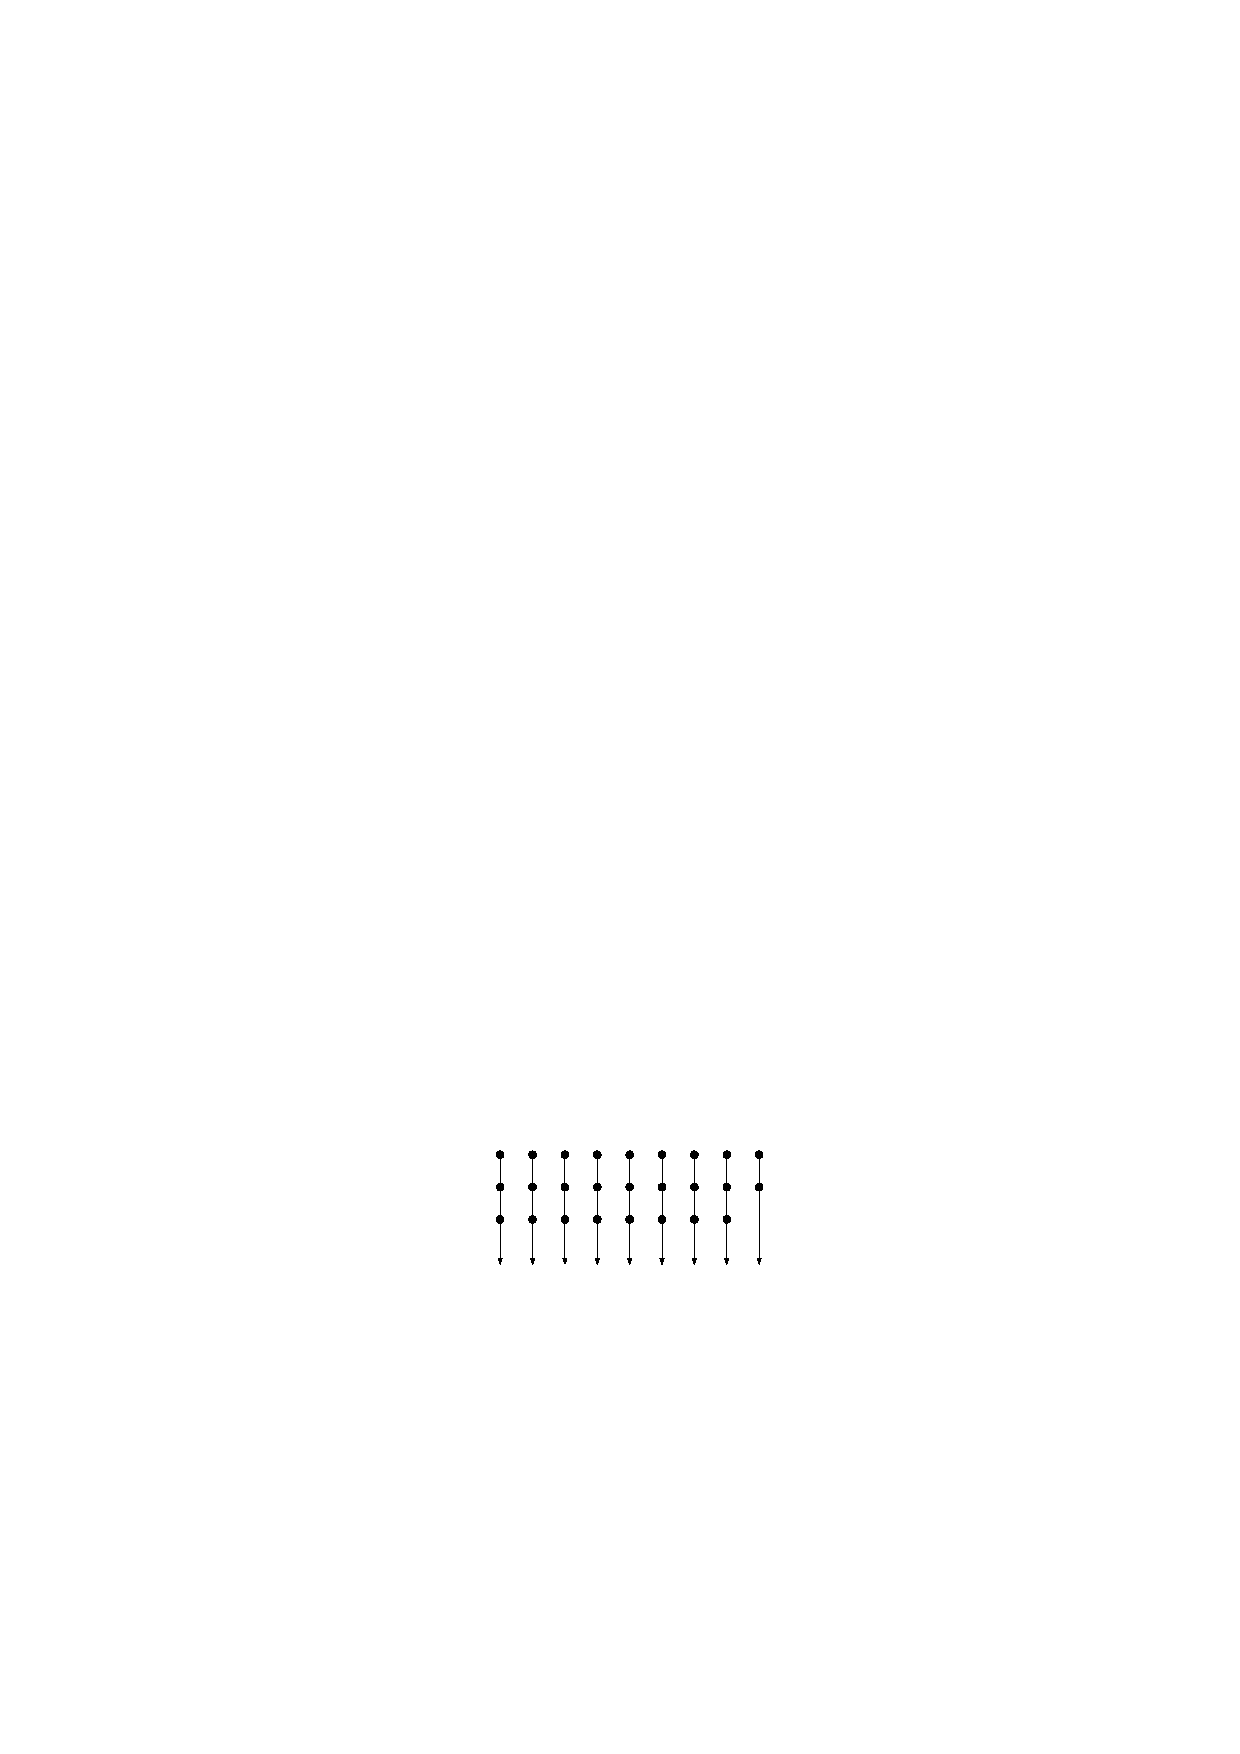
\includegraphics{j0} \\ 
      & $j = 0$  \\
       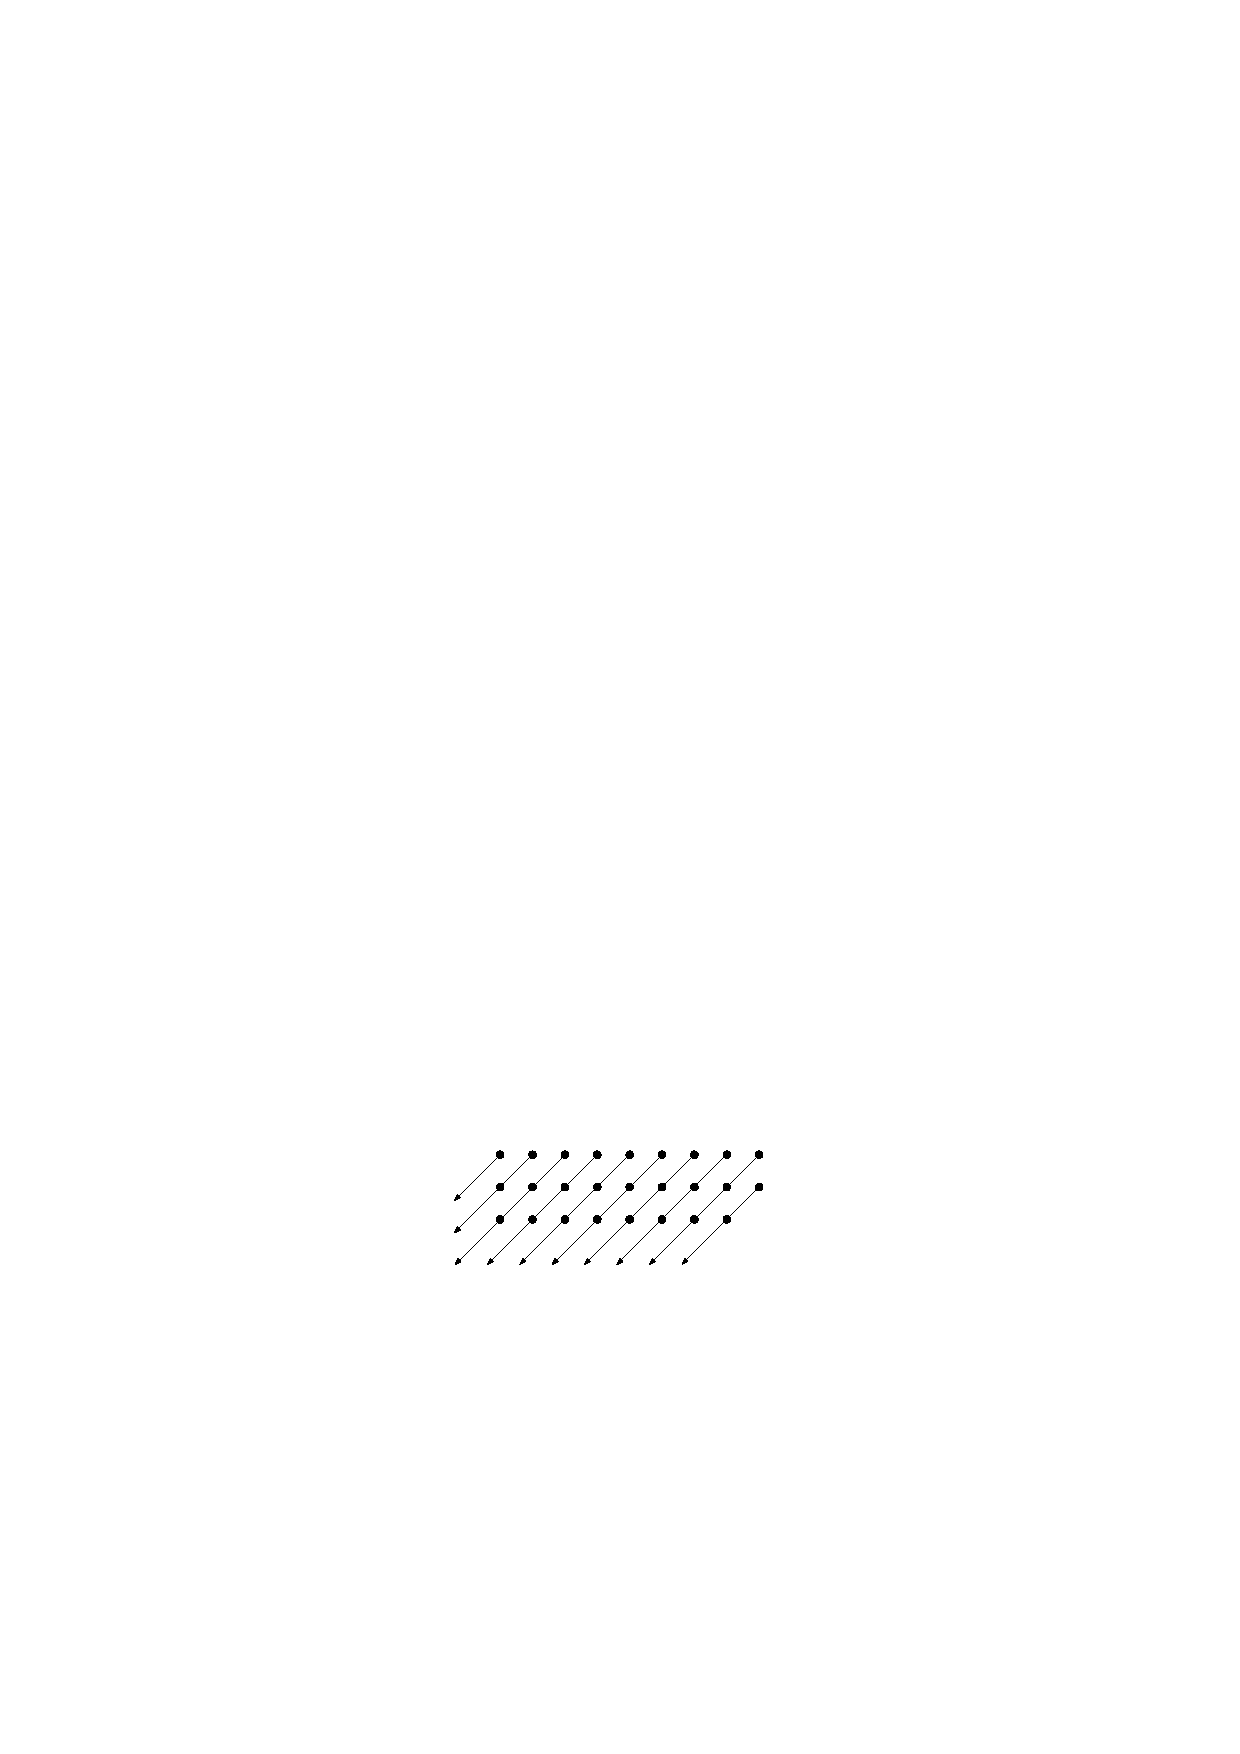
\includegraphics{j1} & 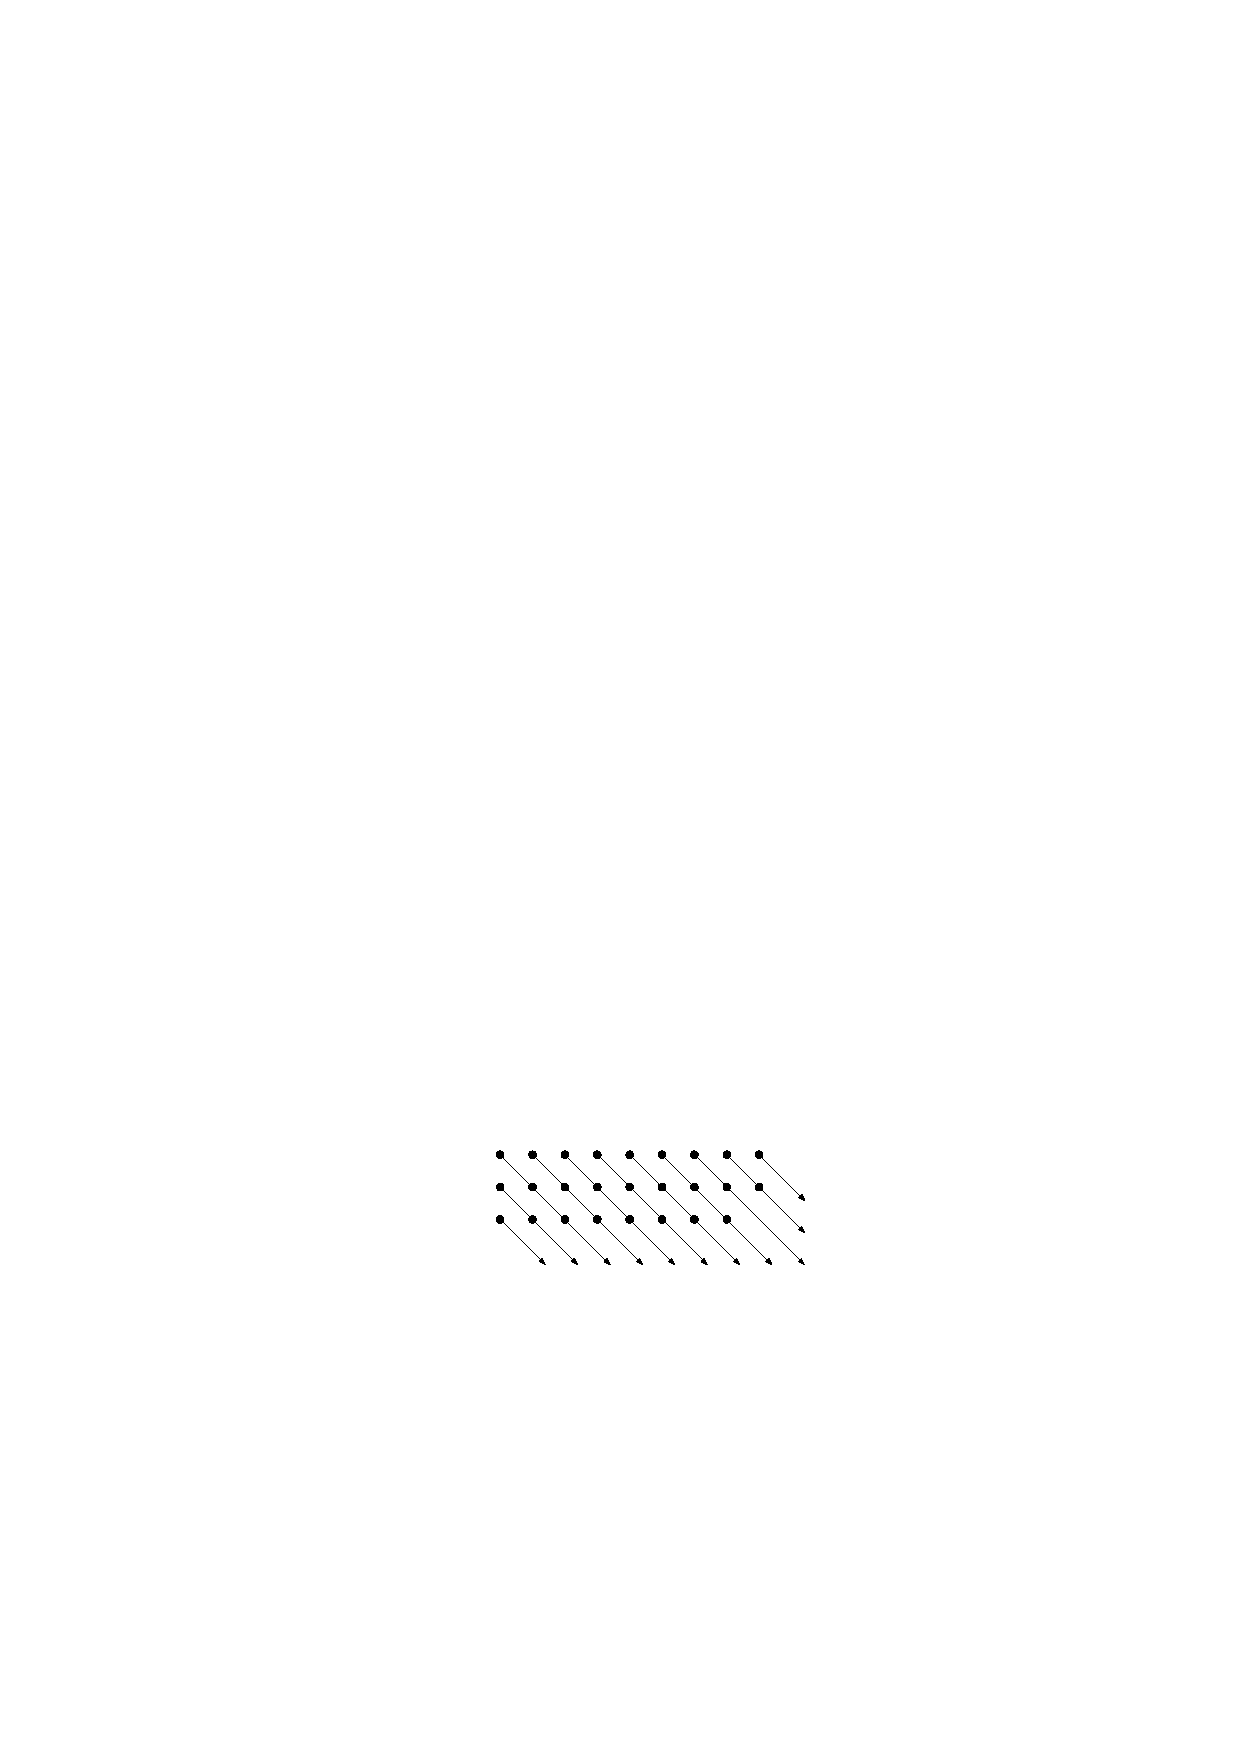
\includegraphics{j2} \\
        $j=1$ & $j=2$ \\
       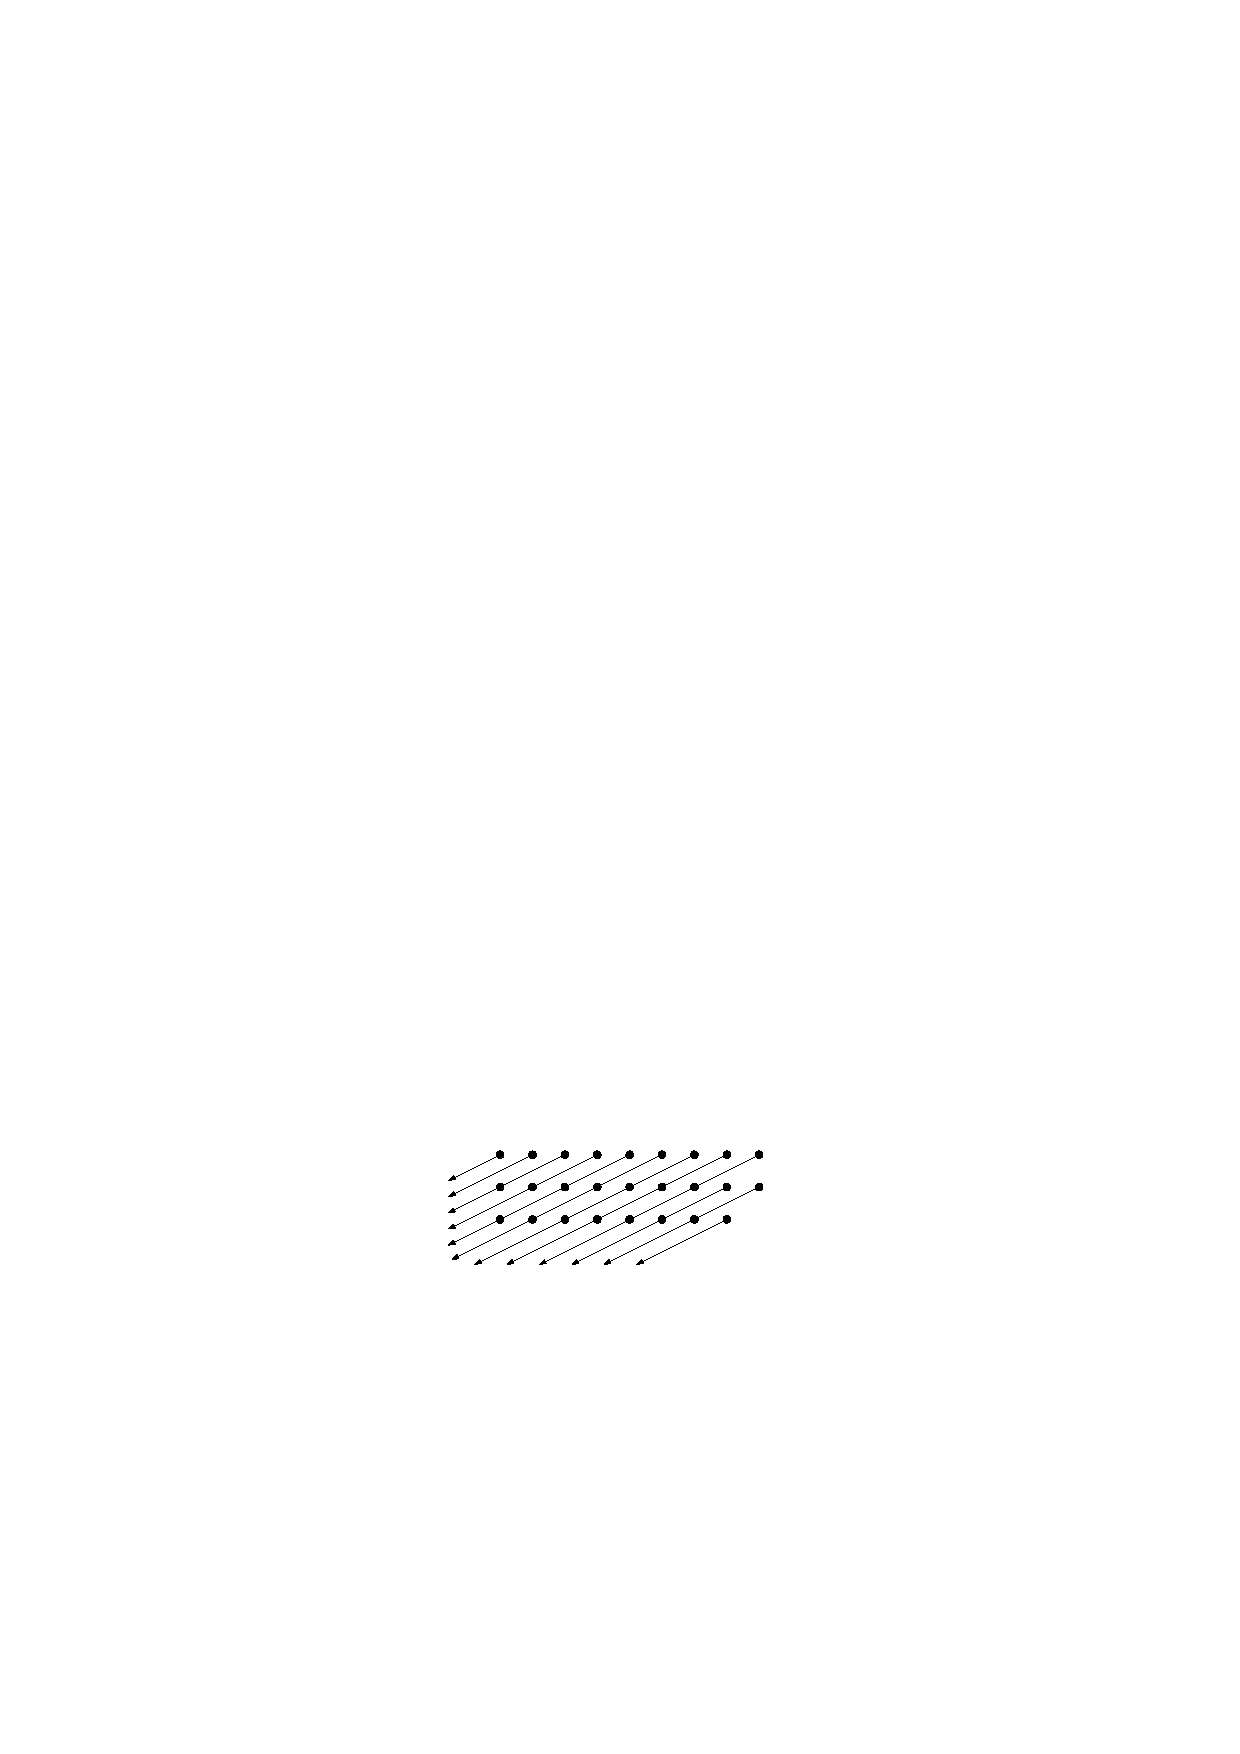
\includegraphics{j3} & 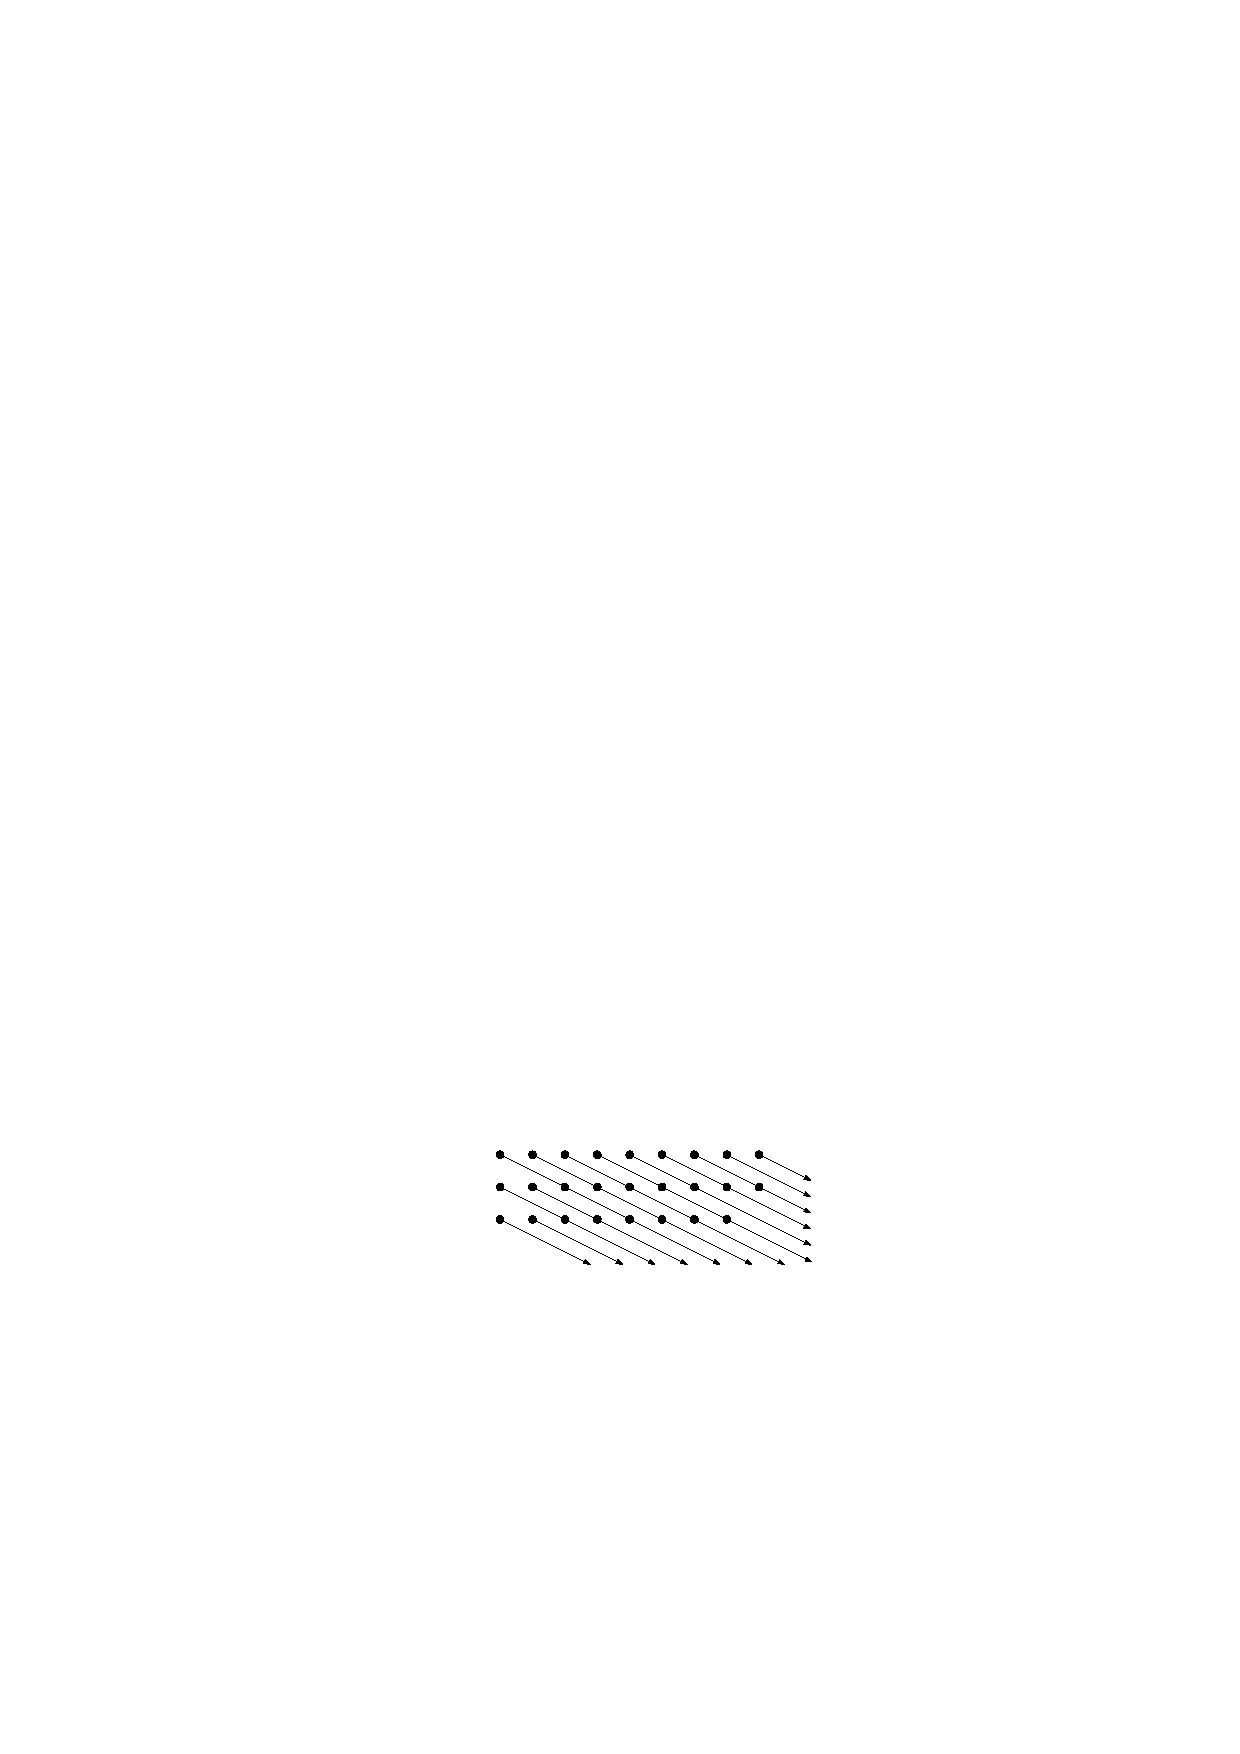
\includegraphics{j4} \\
        $j=3$ & $j=4$
    \end{tabular}
  \end{center}
  \caption{The set $S(i)$  for $i=9$ and the projection directions that yield $i,\ldots,i+4$ distinct points.}
  \figlabel{lower-bound}
\end{figure}
\end{proof}


\section{The Upper Bound}

Our upper-bound proof is closely related to Sz\'ekely's proof of the
Szem\'eredi-Trotter Theorem \cite{s97}.  We make use of the following
version of the Crossing Lemma, which was proven by Pach, Radoici\'c,
Tardos, and T\'oth \cite{prtt04}:

\begin{lem}[Crossing Lemma]\label{lem:crossing}
Let
$\beta=103/6$, $\gamma = 1024/31827$, and let
$G$ be a graph with no self loops, no parallel edges, $v$ vertices, and
$e > \beta v$ edges.  Then
\[
  \cn(G) \ge \gamma \cdot \frac{e^3}{v^2} \enspace .
\]
\end{lem}


\begin{lem}\lemlabel{upper-bound-general}
Let $t=\alpha i$, let $S$ be a set of $r$ points, and let
$H_0,\ldots,H_{t-1}$ be a set of lines such that the orthogonal projection
of $S$ onto $H_{j}$ gives exactly $i+j$ distinct values.  Then, $t\le 34$
or $r\le \max\{4,2/\alpha + 2 + \alpha/2\}i/\gamma$.
\end{lem}

\begin{proof}
Each projection direction $H_j$ defines a set $L_j$ of $i+j$ parallel
lines, each of which contains at least one point of $S$.  Let $G$ be
the geometric graph that contains the points in $S$ plus $t$ additional
points $p_0,\ldots,p_{t-1}$.  Two vertices in $S$ are connected by an
edge in $G$ if and only if they occur consecutively on some line in
$\bigcup_{j=0}^{t-1}L_j$.  Additionally, each vertex $p_j$ is connected
to each of the $i+j$ lexicographically largest points on each of the
lines in $L_j$.  See \figref{graph}.

\begin{figure}
  \begin{center}
    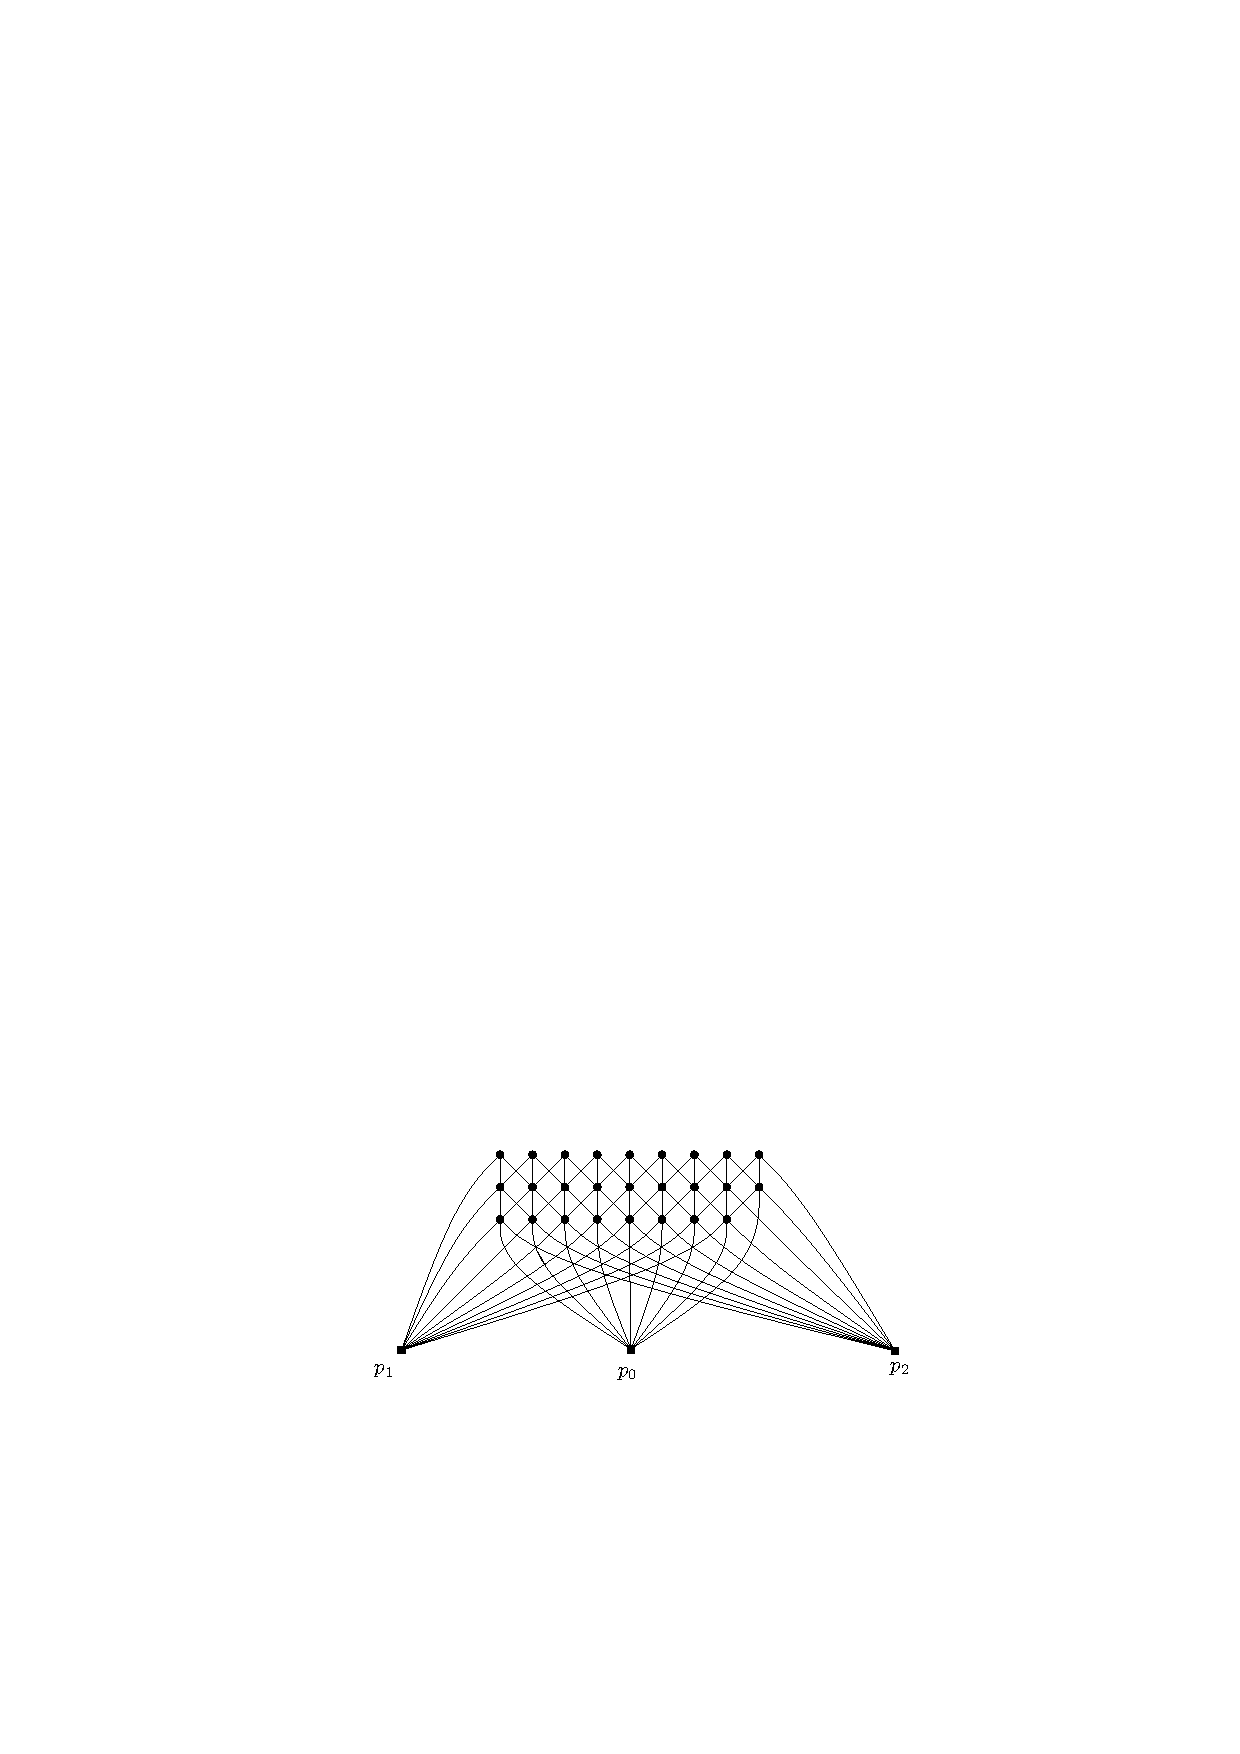
\includegraphics{graph}
  \end{center}
  \caption{The graph $G$ for a set of points with $i=9$ and $t=3$.}
  \figlabel{graph}
\end{figure}

The graph $G$ has $t+r$ vertices
and $tr$ edges.  Observe that we have a drawing of $G$ so that the only
crossings between edges occur where lines in $L$ intersect each other.
The total number of intersecting pairs of lines in $L$ is
\[
  \begin{aligned}
    X 
      & = \sum_{j=1}^{t-1}(i+j)\cdot\sum_{k=0}^{j-1}(i+k) \\
      & \le \sum_{j=1}^{t-1}(i+j)(ij + j^2/2) \\
      & \le \sum_{j=1}^{t-1}(i^2j+3ij^2/2 + j^3/2) \\
      & \le i^2t^2/2 + it^3/2 + t^4/8 \enspace .
  \end{aligned}
\]

Applying \lemref{crossing}, we learn that either
\begin{equation}
   tr \le \beta (t+r) \enspace , \eqlabel{crossing-a}
\end{equation}
or
\begin{equation}
   X \ge \cn(G) \ge \gamma \frac{(tr)^3}{(t+r)^2} \eqlabel{crossing-b} \enspace .
\end{equation}

In the former case, we rewrite \eqref{crossing-a} to obtain
\[
   t \le \beta(t/r + 1) \le 2\beta \le 34 + 1/3 \enspace ,
\]
so $t\le 34$ (since $t$ is an integer).

In the latter case, we expand \eqref{crossing-b} to obtain
\[ i^2t^2/2 + it^3/2 + t^4/8 \ge \gamma\frac{(tr)^3}{(t+r)^2} .  \]
Substituting $t=\alpha i$ gives
\[ i\left(\frac{1}{2\alpha} 
    + \frac{1}{2}+\frac{\alpha}{8}\right) 
      \ge \gamma \frac{r^3}{(t+r)^2} \ge \gamma r/ 4 \enspace ,
\]
where the second inequality follows from the fact that $i+t \le t \le r$.
Rewriting to isolate $r$ finally gives
\[
  r \le \left(\frac{2}{\alpha} + 2 +\frac{\alpha}{2}\right)i/\gamma \enspace .
\]
We finish the proof by observing that, for $\alpha > 2$, the inequality $r\le 4i/\gamma$ obtained by setting $\alpha=2$ is stronger and still applies.
\end{proof}

\begin{lem}\lemlabel{upper-bound}
For all integers $i\ge 1$, $t(i) \le 123.33i+1$.
\end{lem}

\begin{proof}
Observe that $i+t-1\le r$.  Therefore, for $i\ge 18$, the lemma
follows by applying \lemref{upper-bound-general} with $\alpha=2$.
For $i\in\{1,\ldots,17\}$, the lemma follows by setting $\alpha = 35/i$.
\end{proof}

\section{Conclusions}

We have given upper and lower bound on the value of $t$, as a function of
$i$, in an $(i,t)$ set of ghost chimneys.  These bounds differ only by a
(admittedly large) constant factor.  We conjecture that the lower-bound is
tight.  We leave the proof or disproof of this conjecture as an open
problem.

Another open problem is the generalization of these results to 3,
or higher, dimensions: Given an integer $i$, what is the maximum
value $t(i)$ such that there exists a set of points $S\subset\R^d$
and a set $H_0,\ldots,H_{t-1}$ of hyperplanes where, for each
$j\in\{0,\ldots,t(i)-1\}$, the orthogonal projection of $S$ onto $H_j$
consists of exactly $i+j$ distinct points?

\bibliographystyle{plain}
\bibliography{chimneys}



\end{document}
